As Large Language Models (LLMs) continue to advance, efficient inference remains a challenge. Autoregressive decoding generates one token at a time. This inherent seriality creates a major performance bottleneck: decoding is slow, memory-bound, and fails to fully utilize modern GPUs~\citep{cai2024medusa,vaswani2017attention}.

Speculative decoding accelerates a language model, called the \emph{target}, using a smaller model or prediction module, called the \emph{drafter}. The drafter proposes several candidate tokens, and the target checks them in parallel, keeping an accepted prefix and replacing the first rejected proposal with a correction. Appropriate acceptance and correction rules preserve the target's output distribution~\citep{leviathan2023speculative,chen2023sampling}, an idea that goes back to blockwise parallel decoding~\citep{stern2018blockwise} and now covers a broad family of methods~\citep{xia2024survey}. Speedup depends primarily on the length of the accepted prefix in each proposed block, together with the time spent drafting and verifying that block.

Some drafters also use the target's hidden-state representations, which provide contextual information that helps the drafter propose tokens the target will accept. Medusa adds parallel prediction heads to the target's final hidden states~\citep{cai2024medusa}, the EAGLE family uses target features to guide autoregressive drafting~\citep{li2024eagle,li2024eagle2,li2025eagle3}, and DFlash uses a block-diffusion drafter to predict several tokens in one pass, injecting fused target representations into every layer of the drafter model~\citep{chen2026dflash}. Other systems keep the drafter separate and restructure verification instead, using tree-based proposals~\citep{miao2024specinfer,chen2024sequoia}, Jacobi-style decoding~\citep{fu2024lookahead}, or layers of the target itself~\citep{zhang2024draftverify,elhoushi2024layerskip}.

This dependence complicates reuse of the drafter model when a service changes its target's size or family, or fine-tunes it using methods such as LoRA~\citep{hu2022lora}. The new target can produce different hidden states and preferred continuations, and changed feature dimensions may be incompatible with the existing drafter. Training a replacement drafter model requires target-specific supervision, optimization of the drafter's weights, and validation~\citep{li2025eagle3,chen2026dflash}. Repeating this process across target variants increases training and maintenance costs. Can we instead reuse an existing drafter by adapting only its target-feature inputs?

We introduce RelaySpec, a method for reusing a pretrained DFlash drafter~\citep{chen2026dflash} after its target changes (Figure~\ref{fig:relayspec-overview}). Section~\ref{sec:preliminaries} explains the parts of DFlash that RelaySpec uses. The new target supplies hidden states from five layers. A separate linear map transforms each stream before the drafter's original fusion projection combines them. The resulting context conditions the drafter transformer, which predicts a block of candidate tokens.

During adaptation, only the five maps are trained. The target, original fusion projection, drafter transformer, normalization layers, and the embeddings and output head selected for the model pair remain frozen. A map can be rectangular when the target and drafter expect different feature dimensions. Before inference, we multiply each map into its corresponding fusion block, a composition of linear operations. This produces one effective projection, so inference needs no separate mapping operation.

\begin{figure}[t]
    \centering
    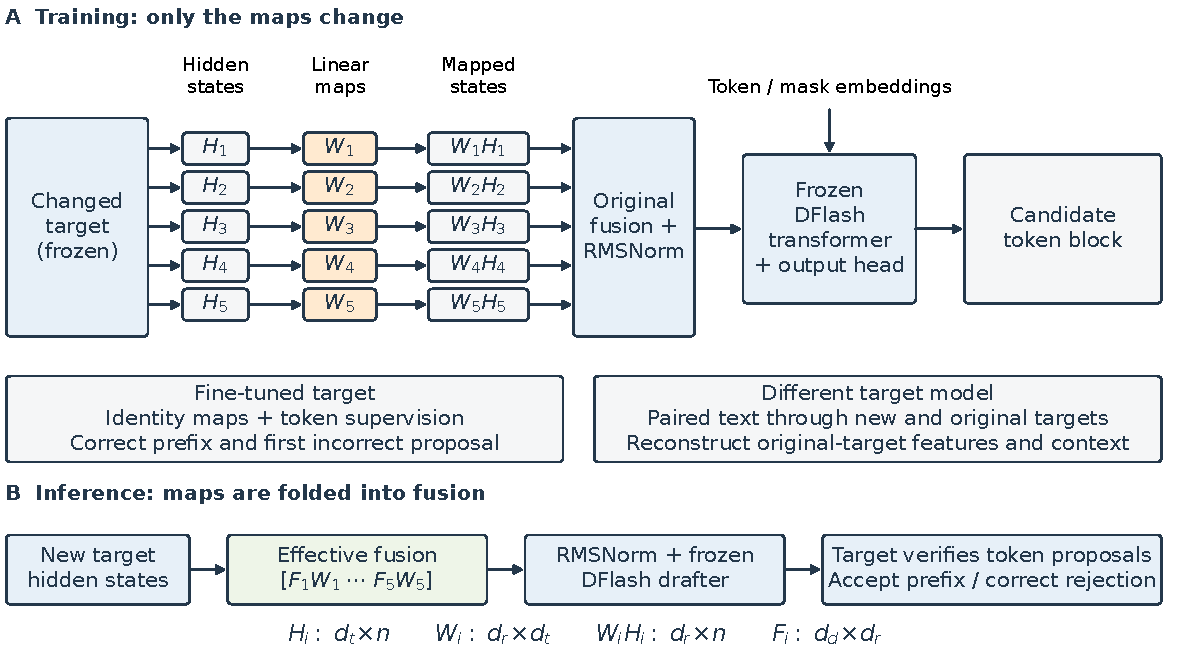
\includegraphics[width=\linewidth]{figures/relayspec_overview.pdf}
    \caption{RelaySpec training and inference. Orange maps are trainable and blue components are frozen. Each hidden-state matrix $H_i$ enters a map $W_i$ before fusion, and a single token gives $W_i h_{i,t}$. For Qwen3-8B with the Qwen3-4B drafter, $d_t=4096$ and $d_r=d_d=2560$, so each $W_i$ is $2560\times4096$ and the folded fusion projection is $2560\times20480$.}
    \label{fig:relayspec-overview}
\end{figure}

RelaySpec uses training signals that match the change in the feature interface: identity-initialized maps trained to improve the accepted prefix for a LoRA-fine-tuned target, and maps that reconstruct the original target's features and fused context for cross-model transfer. Section~\ref{sec:method} gives both procedures.

Our contributions are:
\begin{itemize}
    \item We introduce RelaySpec, an adapter layer between a target model's hidden-state representations and a pretrained DFlash drafter. It uses five trainable linear maps, keeps the drafter transformer frozen, and folds into the original fusion projection before inference.
    \item We evaluate adaptation across fine-tuned targets, model sizes and families, with training-budget and shared-serving comparisons. On Qwen3-4B LoRA targets the selected maps improve mean per-request throughput over the unchanged DFlash drafter by 39.51\% and 85.47\% on GSM8K~\citep{cobbe2021gsm8k} and KiCad. The selected Qwen3-4B-to-8B transfer recovers 100.2\% and 99.4\% of native-drafter throughput on MATH and GSM8K, with weaker transfer on code and chat.
    \item We analyze full-map and correction-map SVD truncation, correction scaling, alignment with LoRA-induced feature changes, and interpolation toward MSE-trained maps.
\end{itemize}
